

{\Large \centering \textbf{Questões e Respostas}\par}


\vspace{20pt}
\section{Questão 4 - Trama de ordem 135}



\subsubsection{Identifique em que frequência do espectro está a operar a rede sem fios, e o canal que corresponde essa frequência.}

    \begin{figure}[H]
    \centering
    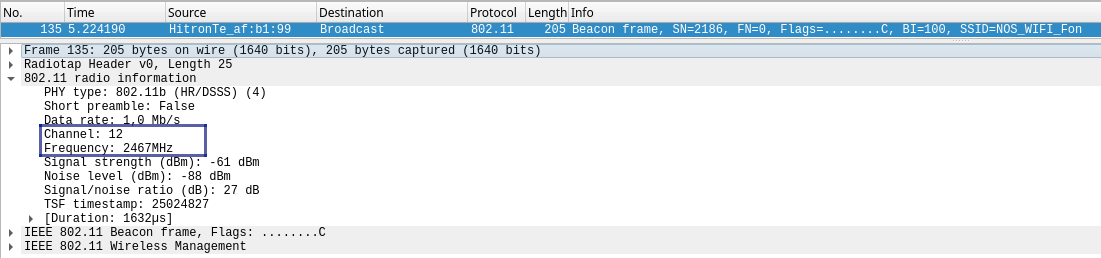
\includegraphics[width=\linewidth]{Prints/Questao4/questao4-1.png}
    \caption{Captura da Trama Nº 135.} \label{questao4-1}
    \end{figure}


    \par Pela Figura \ref{questao4-1}, através do campo \textit{Frequency} conseguimos denotar que a rede sem fios está a operar a \textbf{2467MHz} e, através do campo \textit{Channel} verificamos que corresponde ao canal \textbf{12}.




\vspace{15pt}
\subsubsection{Identifique a versão da norma IEEE 802.11 que está a ser usada.}

%    \begin{figure}[H]
%    \centering
%    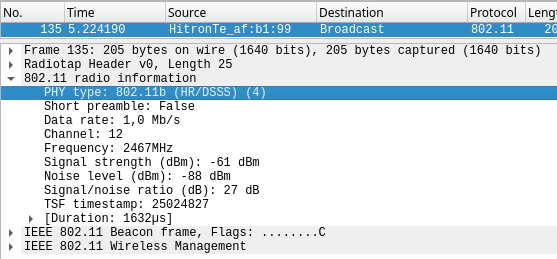
\includegraphics[width=300pt]{Prints/Questao4/questao4-1-802Type.png}
%    \caption{Versão norma IEEE 802.11 usada.} \label{questao4-1-type}
%    \end{figure}


    \par Pela Figura \ref{questao4-1}, no campo \textit{PHY type}, conseguimos denotar a versão da norma IEEE 802.11 que está a ser utilizada, sendo esta a \textbf{802.11b}.




\vspace{15pt}
\subsubsection{Qual o débito a que foi enviada a trama escolhida? Será que esse débito corresponde ao débito máximo a que a interface \textit{Wi-Fi} pode operar? Justifique.}

%    \begin{figure}[H]
%    \centering
%    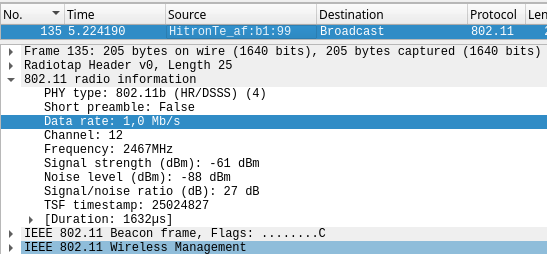
\includegraphics[width=300pt]{Prints/Questao4/questao4-1-Rate.png}
%    \caption{Débito da Trama Nº 135.} \label{questao4-1-type}
%    \end{figure}
    
    
    \par A trama escolhida foi enviada com o débito de \textbf{1.0 Mb/s} (podemos verificar este valor no campo \textit{Data Rate}), no entanto, este débito não corresponde ao débito máximo a que a interface \textit{Wi-Fi} pode operar, uma vez que na versão IEEE 802.11b, o débito máximo é de 11Mb/s.
